\section{Derivation of the Quantitative Model} \label{appendix-model-derivation}

\textit{Given assumptions}:
\begin{enumerate}
    \item Project $Pr$;
    \item Jobs $J$ of project $Pr$;
    \item Jobs $J$ require $N$ nodes, where $N$ is a random variable with expected value $\mu_{N}$ and variance $\sigma_{N}^2$;
    \item Jobs $J$ require walltime $E$, where $E$ is a random variable with expected value $\mu_{E}$ and variance $\sigma_{E}^2$;
    \item Execution times of jobs $J$ equal to their walltime values;
    \item Duration of waiting time in the queue for jobs $J$ is described by a random variable $Q$ with expected value $\mu$ and variance $\sigma^2$;
    \item Jobs $J$ come into the supercomputer queue sequentially: next job is allocated to the queue after the previous one has left the queue to computing nodes.
\end{enumerate}
\textit{Values to find}:
$P(U > U_0)$ - the probability that utilization $U$ during the time interval $T_0$ will exceed the predefined value $U_0$, where $T_0$ is big.

\textit{Solution}.
Using the Law of total probability we can write the following equation:
\begin{equation}
    \label{eq-1}
    P(U > U_0) = \sum\limits_{n=1}^{\infty}P(U(n) > U_0) P(n)
\end{equation}
where $U(n)$ is a random variable for utilization achieved by $n$ sequential jobs $J$; $P(n)$ is a probability that during the time $T_0$ exactly $n$ jobs $J$ will be running. We assume that $T_0$ is big, so values of $P(n)$ for the first several $n$ (e.g., for $n$ from 1 to 99) are equal to zero, thus the sum would start with $n=100$.

To calculate $P(n)$ let's consider a random variable $T(n)$ describing the time required to run $n$ sequential jobs $J$. Taking into account one of the assumptions (6) we can write:
\begin{equation}
    \label{eq-2}
    T(n) = \sum\limits_{i=1}^{n}Q_{i}
\end{equation}
where $Q_{i} = Q$ is a random variable describing duration of waiting time in the queue for the job $J_{i}$. And, using Central limit theorem we can write for big values of $n$:
\begin{equation}
    \label{eq-3}
    \sum\limits_{i=1}^{n}Q_{i} \approx N(n\mu, n\sigma^2)
\end{equation}
where $N(\mu, \sigma^2)$ is a normal distribution with expected value $\mu$ and variance $\sigma^2$; $\mu$ is an expected value of a random variable $Q$ describing duration of waiting time in the queue for jobs $J$; $\sigma^2$ is a variance of a random variable $Q$ describing duration of waiting time in the queue for jobs $J$.

The probability $P(n)$ can be rewritten as following:
\begin{equation}
    \label{eq-4}
    P(n_0) = P(n \geq n_0) - P(n \geq n_0 + 1)
\end{equation}
where $P(n_0)$ is a probability that during the time $T_0$ precisely $n_0$ jobs $J$ will be running; $P(n \geq n_0)$ is a probability that during the time $T_0$ not less than $n_0$ jobs $J$ will be running. We can mention that the event $n \geq n_0$ (during the time $T_0$ not less than $n_0$ jobs $J$ will be running) is equal to the event $T(n_0) \leq T_0$ (the time required to run $n_0$ jobs $J$ is less than or equal to the time $T_0$). Considering that we have: $P(n \geq n_0) = P(T(n_0) \leq T_0)$ and $P(n \geq n_0 + 1) = P(T(n_0 + 1) \leq T_0)$. Thus, inserting these equations into Equation \ref{eq-4} and using Equations \ref{eq-2} and \ref{eq-3} we can have the following:
\begin{equation}
    \label{eq-5}
    \begin{multlined}
    P(n_0) = P(N(n_0\mu, n_0\sigma^2) \leq T_0) \  - \\
             \shoveleft[1cm]{P(N((n_0 + 1)\mu, (n_0 + 1)\sigma^2) \leq T_0)}
    \end{multlined} 
\end{equation}

This equation can be updated by using the probability density of the normal distribution:
\begin{equation}
    \label{eq-6}
    \begin{multlined}
    P(n_0) = \int_{-\infty}^{T_0}f(x, n_0\mu, n_0\sigma^2)dx \  - \\
             \shoveleft[1cm]{\int_{-\infty}^{T_0}f(x, (n_0 + 1)\mu, (n_0 + 1)\sigma^2)dx}
    \end{multlined}
\end{equation}
where $f(x, \mu, \sigma^2)$ is a function of probability density of the normal distribution $N(\mu, \sigma^2)$.

To calculate value of $P(U(n) > U_0)$ in Equation \ref{eq-1} let's write a random variable $U(n)$ as a sum of random variables $U_{i}$ describing utilization of the single job $J_{i}$: $U(n_0) = \sum_{i=1}^{n_0}U_{i}$. Assuming that all random variables $U_{i}$ have the same expected values (let's denote them as $\mu_{U}$) and variances (let's denote them as $\sigma_{U}^2$) and using as before the Central limit theorem we can write for big values of $n$:
\begin{equation}
    \label{eq-7}
    U(n_0) = \sum_{i=1}^{n_0}U_{i} \approx N(n_0\mu_{U}, n_0\sigma_{U}^2)
\end{equation}

Using the probability density of the normal distribution and Equation \ref{eq-7} we can write $P(U(n) > U_0)$ in a way:
\begin{equation}
    \label{eq-8}
    P(U(n) > U_0) = \int_{U_0}^{\infty}f(x, n\mu_{U}, n\sigma_{U}^2)dx
\end{equation}

To get the final equation we insert Equations \ref{eq-6} and \ref{eq-8} into the Equation \ref{eq-1}:
\begin{equation}
    \label{eq-9}
    \begin{multlined}
    P(U > U_0) = \sum\limits_{n=100}^{\infty} 
                 \bigg[ \int_{U_0}^{\infty}f(x, n\mu_{U}, n\sigma_{U}^2)dx \  \times \\
                 \bigg( \int_{-\infty}^{T_0}f(x, n\mu, n\sigma^2)dx \  - \\
                 \int_{-\infty}^{T_0}f(x, (n+1)\mu, (n+1)\sigma^2)dx \bigg) \bigg]
    \end{multlined}
\end{equation}

The outcome of the Equation~\ref{eq-9} is the probability that the utilization of resources, which is achieved by a sequential set of processed jobs using capabilities of the supercomputer during the time interval $T_0$, is greater than the predefined value $U_0$. It implies that:
\begin{itemize}
	\item Utilization of every single job is described by a random variable with the expected value $\mu_{U}$ and the variance $\sigma_{U}^2$;
	\item The time interval between launches of sequential jobs is described by a random variable with the expected value $\mu$ and the variance $\sigma^2$.
\end{itemize}

Generally, the distribution of a random variable that describes the size of the job in a way as the number of occupied cores (denote this random variable as $N$) and the distribution of a random variable that describes the time to complete for a single job (denote this random variable as $E$) are more commonly known compare to the distribution of a random variable that describes the utilization achieved by a single job (denote this random variable as $U$). Since, the utilization of a single job is a product of the amount of the used resources by the time to complete this job, then, in case of mutual independence of random variables $N$ and $E$, the values $\mu_U$ and $\sigma_{U}^2$ can be found by the following equations:
\begin{equation}
    \label{eq-10}
    \mu_U = \mu_N \mu_E \\
\end{equation}
where $\mu_N$ is the expected value of the random variable $N$; $\mu_E$ is the expected value of the random variable $E$.
\begin{equation}
    \label{eq-11}
    \sigma_{U}^2 = \sigma_{N}^2 \sigma_{E}^2 + \mu_N \sigma_{E}^2 + \mu_E \sigma_{N}^2
\end{equation}
where $\sigma_{N}^2$ is the variance of the random variable $N$; $\sigma_{E}^2$ is the variance of the random variable E.


\section{Description of the Simulator} \label{appendix-simulator-description}

The simulator is based on the Queueing Theory~\cite{ref-queueing-theory} and
according to the Kendall's Notation~\cite{ref-kendall} for queues, usually
referred as A/B/C/D/E, it is characterized as following:
\begin{itemize}
    \item A - \textit{arrival process} is represented by streams that are
    responsible for job generation and is described either by a Poisson
    process or by a deterministic model;
     \item B - \textit{service/server process} is represented by a set of
    nodes that simulate job execution process and is described either by a
    Poisson process or by a deterministic model as well;
    \item C - \textit{number of servers} that corresponds to the number of
    compute nodes (in terms of the Titan supercomputer);
    \item D - \textit{capacity of the queue or system overall}, which is
    ``on'', if the queue limit is set (either per stream or for the total
    number of jobs in the queue) and queue buffer is not used, otherwise the
    capacity is unlimited;
    \item E - \textit{queueing discipline} is provided in two options: FIFO
    or Priority.
\end{itemize}

Some of the parameters are set as requirements and restrictions applied to a
specific supercomputer and its policy, e.g., the total number of compute
nodes that are available for computing jobs, the limit of the number of jobs
in the queue per user/group, etc.

\subsection{General Overview} \label{appendix-simulator-description-1}

Implementation of the simulator (Queueing System Simulator) \cite{ref-qss}
was done by using Python\footnote{High-level programming language Python,
\url{https://docs.python.org/2.7/} [accessed on 2020-01-10]}, and the
following key classes and generators were designed (to emulate internal
supercomputer processes):
\begin{itemize}
    \item \textit{Job} - contains parameters to describe job's processing
    life-cycle, such as arrival timestamp, start execution timestamp,
    completion timestamp that is based on wall time / execution time along
    with the previous parameter, number of required nodes for its execution,
    stream (i.e., source name), label (i.e., project name), priority and
    priority group name;
    \item \textit{Stream} - generates jobs with the predefined parameters as
    an input for the simulator;
    \item \textit{Queue Manager} - emulates buffer ahead of the queue, the
    queue itself, and manages jobs while waiting for their execution, it
    lets to define the queue discipline such as FIFO and Priority, and set
    the limits per input job stream;
    \item \textit{Schedule Manager} - emulates a back-fill mode - gets
    information about job sizes, assigns corresponding nodes for execution,
    gives a schedule when each job starts to be executed;
    \item \textit{QSS} - the core class that manages and tracks job's
    processing life-cycle.
\end{itemize}

\subsection{Job State Model} \label{appendix-simulator-description-2}

Job life-cycle (in terms of the simulator, Figure~\ref{fig-simulator-scheme})
includes the following states: \textbf{Generated} - \textbf{Holding} (i.e.,
Titan notation: blocked) [buffer] - \textbf{Pending} (i.e., Titan notation:
eligible-to-run) [queue] - \textbf{Starting} - \textbf{Executing} -
\textbf{Finished}.
Some of the states might be skipped if certain components are turned off (e.g.,
if the queue buffer is not used then there is no state ``holding'') or if there
is some initial restriction (e.g., state ``starting'' is neglected, since the
assumption that job execution starts right after it leaves the queue).

\begin{figure}
    \centering
    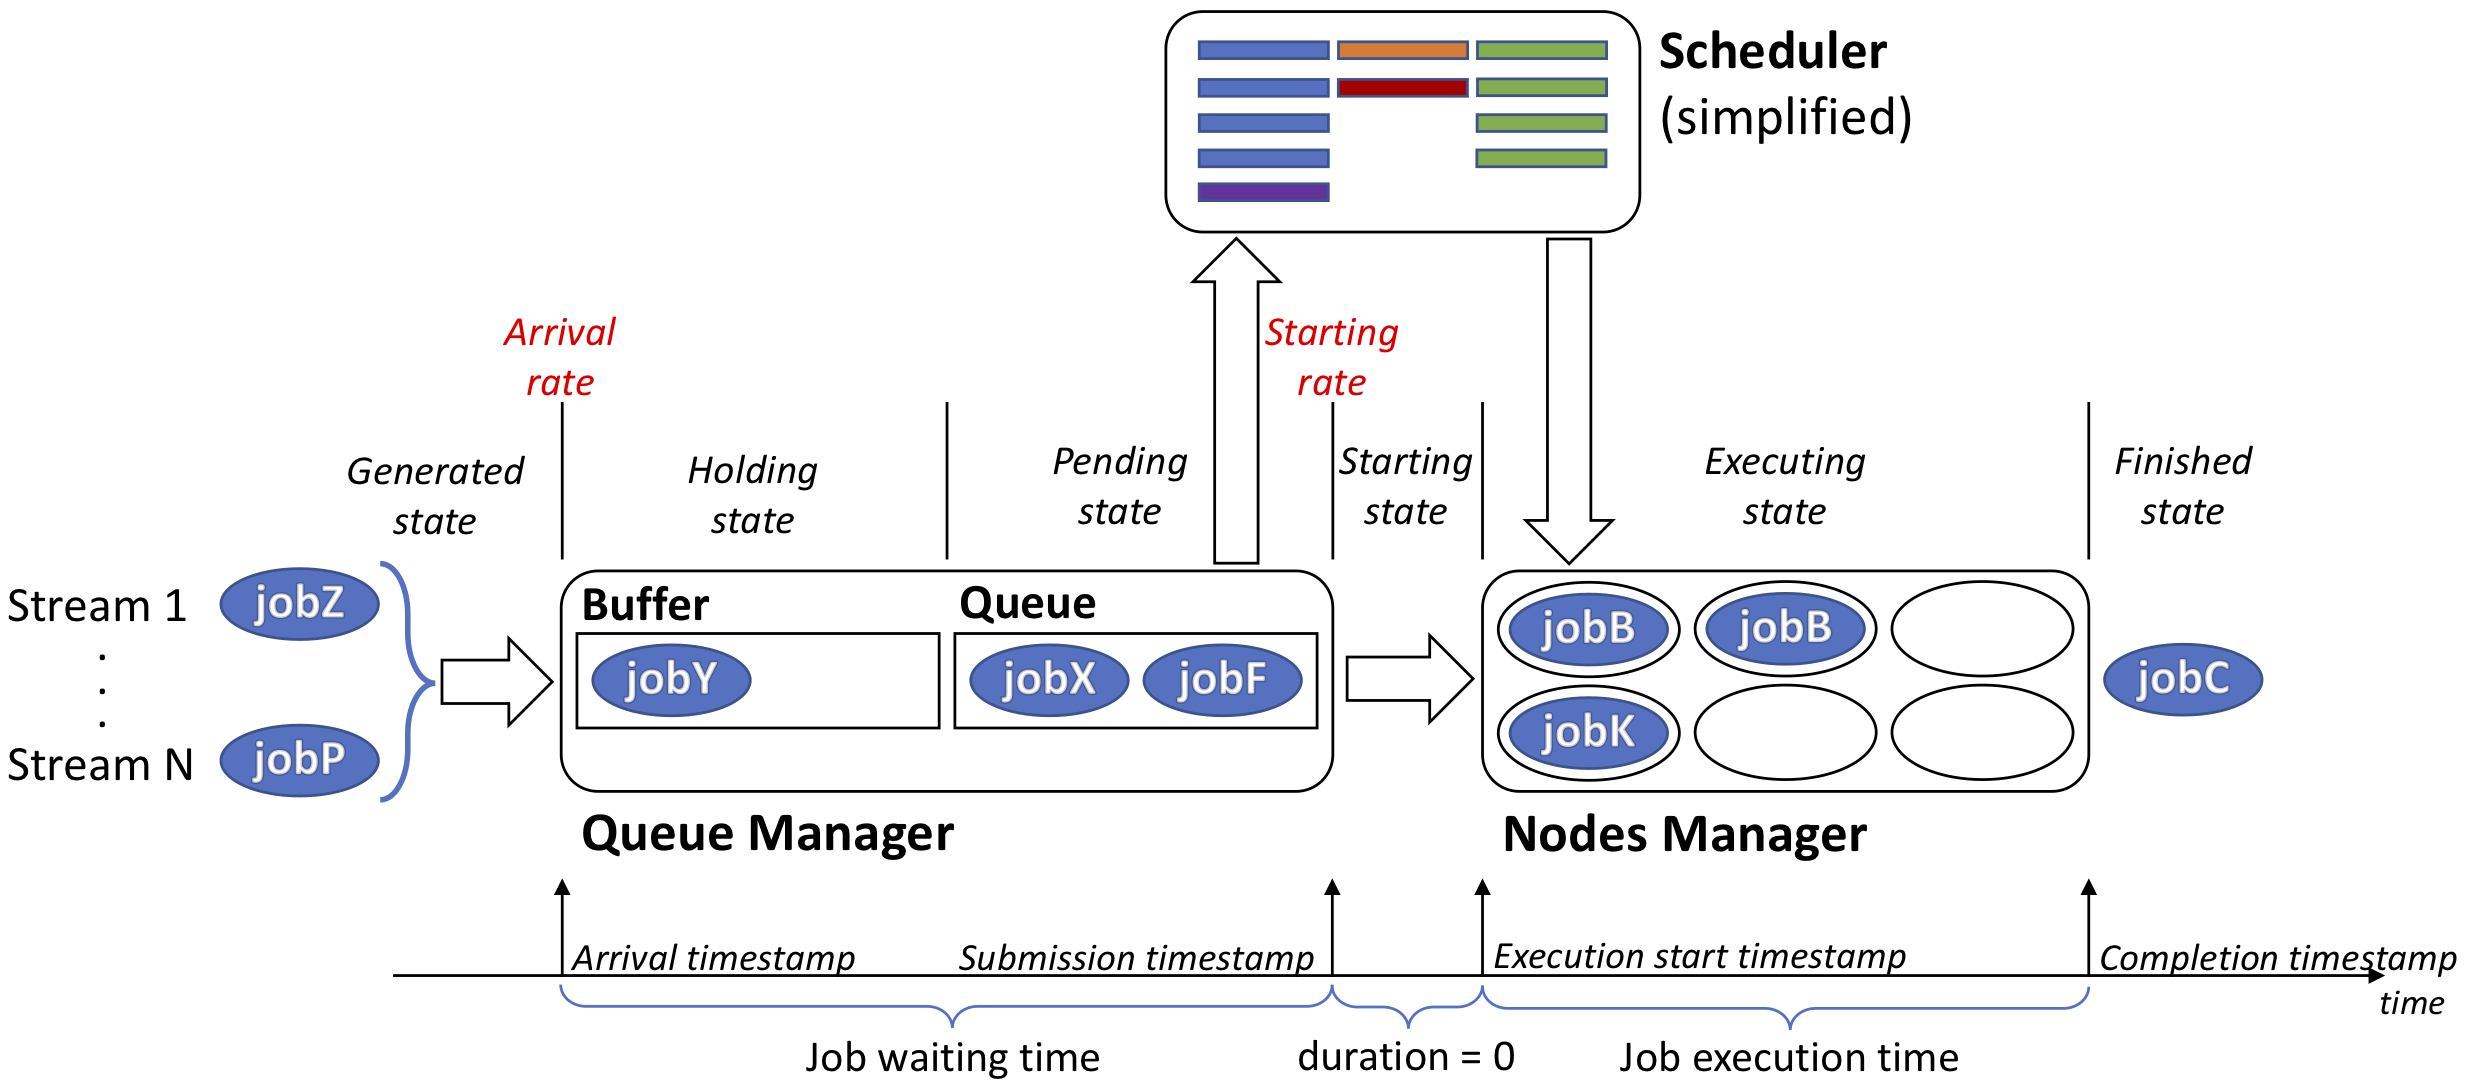
\includegraphics[width=0.48\textwidth]{pics/simulator-scheme.png}
    \caption{Job state transitions at the simulator}
    \label{fig-simulator-scheme}
\end{figure}
